\documentclass{beamer}
\usepackage[utf8]{inputenc}

\usetheme{Madrid}
\usecolortheme{default}
\usepackage{txfonts}
\usepackage{listings}
\usepackage{adjustbox}
\usepackage{tabularx}
\usepackage{lmodern}
\usepackage{circuitikz}
\usepackage{tikz}

\usepackage{gvv}
\usepackage{cite}
\usepackage{amsmath,amssymb,amsfonts,amsthm}
\usepackage{algorithmic}
\usepackage{graphicx}
\usepackage{textcomp}
\usepackage{xcolor}
\usepackage{txfonts}
\usepackage{listings}
\usepackage{enumitem}
\usepackage{mathtools}
\usepackage{gensymb}
\usepackage{comment}
\usepackage{tkz-euclide} 
\usepackage{listings}                                      
\def\inputGnumericTable{}                                
\usepackage{color}                                            
\usepackage{array}                                            
\usepackage{longtable}
\usepackage{multicol}
\usepackage{calc}                                             
\usepackage{multirow}                                         
\usepackage{hhline}                                           
\usepackage{ifthen}

\setbeamertemplate{page number in head/foot}[totalframenumber]

\usepackage{tcolorbox}
\tcbuselibrary{minted,breakable,xparse,skins}



\definecolor{bg}{gray}{0.95}
\DeclareTCBListing{mintedbox}{O{}m!O{}}{%
  breakable=true,
  listing engine=minted,
  listing only,
  minted language=#2,
  minted style=default,
  minted options={%
    linenos,
    gobble=0,
    breaklines=true,
    breakafter=,,
    fontsize=\small,
    numbersep=8pt,
    #1},
  boxsep=0pt,
  left skip=0pt,
  right skip=0pt,
  left=25pt,
  right=0pt,
  top=3pt,
  bottom=3pt,
  arc=5pt,
  leftrule=0pt,
  rightrule=0pt,
  bottomrule=2pt,
  toprule=2pt,
  colback=bg,
  colframe=orange!70,
  enhanced,
  overlay={
    \begin{tcbclipinterior}
    \fill[orange!20!white] (frame.south west) rectangle ([xshift=20pt]frame.north west);
    \end{tcbclipinterior}},
  #3,
}
\lstset{
    language=C,
    basicstyle=\ttfamily\small,
    keywordstyle=\color{blue},
    stringstyle=\color{orange},
    commentstyle=\color{green!60!black},
    numbers=left,
    numberstyle=\tiny\color{gray},
    breaklines=true,
    showstringspaces=false,
}

\title 
{1.5.19}
\date{August 29, 2025}


\author 
{Sai Sreevallabh - EE25BTECH11031}



\begin{document}


\frame{\titlepage}
\begin{frame}{Question}
Find the ratio in which the segment joining the points $\brak{1,3}$ and $\brak{4,5}$ is divided by the X-axis. Also find the coordinates of this point on the X-axis.
\end{frame}



\begin{frame}{Theoretical Solution}

Given points are\\
\begin{align}
    \vec{A}=\myvec{1\\3} \ \text{and}\  \vec{B}=\myvec{4\\5}
\end{align}

Let $\vec{P}$ be a point on the x-axis. We can assume it to be\\

\begin{align}
    \vec{P}=\myvec{x\\0}
\end{align}

\end{frame}


\begin{frame}{Theoretical Solution}

$\vec{A}$, $\vec{B}$ and $\vec{P}$ are collinear. 

\begin{align}
    \vec{P}-\vec{A}=\myvec{x-1 \\ -3} \ , \ 
    \vec{B}-\vec{A}=\myvec{3\\2}  
\end{align}

\begin{align}
    \myvec{\vec{P}-\vec{A} & \vec{B}-\vec{A}}^T =& \myvec{x-1 & 3\\ -3 & 2}^T\\
    =& \myvec{x-1 & -3 \\ 3 & 2}
\end{align}

\end{frame}

\begin{frame}{Theoretical Solution}

Converting into echelon form using row operations

\begin{align*}
    \myvec{x-1 & -3 \\ 3 & 2}\ \xleftrightarrow[]{R_2 \to R_2-\frac{3}{x-1}R_1} \  \myvec{x-1 & -3 \\ 0 & \frac{2x+7}{x-1}}
\end{align*}

Since the points are collinear, we can say that the rank of the matrix is $1$ i.e. 

\begin{align}
    &\frac{2x+7}{x-1} = 0\\
    \implies& x=-\frac{7}{2}
\end{align}

\end{frame}

\begin{frame}{Theoretical Solution}
Let $\vec{P}$ divide the line joining points $\vec{A}$ and $\vec{B}$ in the ratio $k:1$. 

\begin{align}
    \vec{P}=\frac{k\vec{B}+\vec{A}}{k+1}
\end{align}

\begin{align}
    k\brak{\vec{P}- \vec{B}} = \vec{A}-\vec{P}
\end{align}

\end{frame}

\begin{frame}{Theoretical Solution}

\begin{align}
    k=\frac{\brak{\vec{P}-\vec{B}}^T\brak{\vec{A}-\vec{P}}}{||\brak{\vec{P}-\vec{B}}||^2}
\end{align}

\begin{align}
      k=\frac{\myvec{x-4 & -5}\myvec{1-x\\3}}{{\norm{\myvec{x-4 \\ -5}}}^2}
\end{align}

\end{frame}

\begin{frame}{Theoretical Solution}
    Substituting the value of $x$ as $-\frac{7}{2}$, we get the value of k as

\begin{align}
    k=-\frac{3}{5}
\end{align}

Therefore,\\

The point $\vec{P}\myvec{-\frac{7}{2}\\0}$ on the X-axis divides the line segment in the ratio $-3:5$ i.e. externally in the ratio $3:5$.
\end{frame}

\begin{frame}[fragile]
    \frametitle{C Code - Function to Find x Coordinate of P}

    \begin{lstlisting}

#include <stdio.h>
#include <math.h>

float Solve_for_x(float x1, float y1, float x2, float y2){

//assuming that the point divides the line in ratio k:1

	float k = -y1/y2;
	float x = (x1+k*x2)/(k+1);

	return x;
}
    \end{lstlisting}

\end{frame}

\begin{frame}[fragile]
    \frametitle{Python Code - Using Shared Object}
    \begin{lstlisting}
import sys
import math
import numpy as np
import matplotlib.pyplot as plt
import ctypes
import numpy.linalg as LA

c_lib=ctypes.CDLL("./code.so")

c_lib.Solve_for_x.argtypes = [
        ctypes.c_float,
        ctypes.c_float,
        ctypes.c_float,
        ctypes.c_float
        ]
c_lib.Solve_for_x.restype = ctypes.c_float
\end{lstlisting}
\end{frame}

\begin{frame}[fragile]
    \frametitle{Python Code - Using Shared Object}
    \begin{lstlisting}
A= np.array([1,3]).reshape(-1,1)
B= np.array([4,5]).reshape(-1,1)

x = c_lib.Solve_for_x(
        ctypes.c_float(A[0]),
        ctypes.c_float(A[1]),
        ctypes.c_float(B[0]),
        ctypes.c_float(B[1])
        )

#P is the point on X-axis that divides the given line segment in the ratio k:1

P = np.array([x,0]).reshape(-1,1)

\end{lstlisting}
\end{frame}

\begin{frame}[fragile]
    \frametitle{Python Code - Using Shared Object}
    \begin{lstlisting}
    
plt.plot([P[0,0], B[0,0]], [P[1,0], B[1,0]], label="Line Segment AB (Extended to P)")

plot_coords = np.block([[A, B, P]])
plt.scatter(plot_coords[0,:], plot_coords[1,:], color="red")


vert_labels = [
    f'A({A[0,0]}, {A[1,0]})',
    f'B({B[0,0]}, {B[1,0]})',
    f'P({P[0,0]:.2f}, {P[1,0]})'
]

\end{lstlisting}
\end{frame}

\begin{frame}[fragile]
    \frametitle{Python Code - Using Shared Object}
    \begin{lstlisting}
for i, txt in enumerate(vert_labels):
    plt.annotate(txt,
            (plot_coords[0,i],plot_coords[1,i]),
            textcoords="offset points",
            xytext=(0,10),
            ha='center')

plt.xlabel('$x$')
plt.ylabel('$y$')
plt.title("Line Segment AB Divided by X-axis")
plt.legend(loc='upper left')
plt.grid()
plt.axis('equal')

plt.savefig("../Figs/plot(py+C).png")

plt.show()
\end{lstlisting}
\end{frame}

\begin{frame}{Plot-Using Both C and Python}
    \centering
    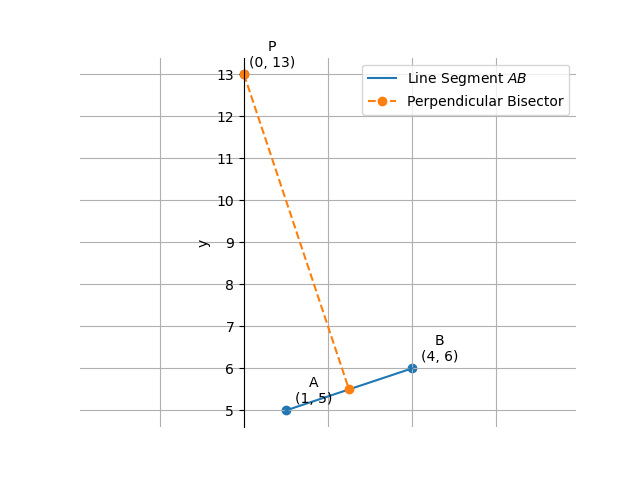
\includegraphics[width=\columnwidth, height=0.8\textheight, keepaspectratio]{Figs/plot(py+C).png}     
\end{frame}

%-------End of Python+C-------------


\begin{frame}[fragile]
    \frametitle{Python Code}
    \begin{lstlisting}
import sys
import math
sys.path.insert(0, '/home/sai-sreevallabh/Matrix_Theory/Matgeo/codes/CoordGeo')
import numpy as np
import matplotlib.pyplot as plt
import matplotlib.image as mpimg
import numpy.linalg as LA

#local imports
from line.funcs import *
from triangle.funcs import *

#if using termux
import subprocess
import shlex

\end{lstlisting}
\end{frame}

\begin{frame}[fragile]
    \frametitle{Python Code}
    \begin{lstlisting}
A = np.array([1,3])
B = np.array([4,5])

k = -(A[1])/(B[1])

x = (A[0] + k*B[0])/(k+1)
x = np.round(x,1)

P = np.array([x,0.0])

A = A.reshape(-1,1)
B = B.reshape(-1,1)
P = P.reshape(-1,1)
\end{lstlisting}
\end{frame}

\begin{frame}[fragile]
    \frametitle{Python Code}
    \begin{lstlisting}
x_PB = line_gen_num(P, B, 20)
plt.plot(x_PB[0,:],x_PB[1,:], color='green', label="Line Segment AB (Extended to P)")

plot_coords = np.block([[A, B, P]])
plt.scatter(plot_coords[0,:], plot_coords[1,:], color='red')

vert_labels = [
    f'A({A[0,0]}, {A[1,0]})',
    f'B({B[0,0]}, {B[1,0]})',
    f'P({P[0,0]:.2f}, {P[1,0]})'
]
\end{lstlisting}
\end{frame}

\begin{frame}[fragile]
    \frametitle{Python Code}
    \begin{lstlisting}
for i, txt in enumerate(vert_labels):
    plt.annotate(txt,
            (plot_coords[0,i], plot_coords[1,i]),
            textcoords="offset points",
            xytext=(0,10),
            ha='center')

plt.xlabel('$x$')
plt.ylabel('$y$')
plt.title("Line Segment AB Divided by X-axis")
plt.legend(loc='upper left')
plt.grid()
plt.axis('equal')

plt.savefig("../Figs/plot(py).png")
plt.show()
    \end{lstlisting}
\end{frame}


\begin{frame}{Plot-Using Python only}
    \centering
    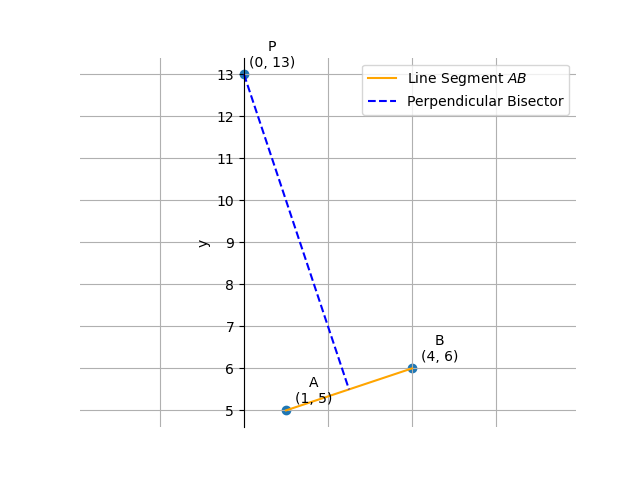
\includegraphics[width=\columnwidth, height=0.8\textheight, keepaspectratio]{Figs/plot(py).png}     
\end{frame}


\end{document}
